% !TeX encoding = UTF-8 Unicode
\documentclass[a4paper,12pt]{article}
\usepackage[english]{babel}
\usepackage[english]{isodate}
\usepackage{graphicx}
\usepackage{hyperref}
\usepackage{centernot}
\usepackage{xfrac}
\usepackage{mathtools}
\usepackage{enumitem}
\usepackage{fancyhdr}
\usepackage{lastpage}
\usepackage{xcolor}
\usepackage{changepage}
\usepackage{amsthm}
\usepackage{amsfonts}
\usepackage{amsmath}
\usepackage{amssymb}
\usepackage{soul}
\usepackage{float}
\usepackage{centernot}
\usepackage{tcolorbox}
\usepackage{titling}
\usepackage{caption}
\usepackage{subcaption}
\usepackage{etoolbox}
\usepackage{listings}
\usepackage{biblatex}
\usepackage{csquotes}
\usepackage{titlesec}
\usepackage{tikz}

\addbibresource{bibliography.bib}

%https://github.com/diku-dk/futhark/blob/master/tools/futhark-listings.tex
\lstdefinelanguage{futhark}
{
  % list of keywords
  morekeywords={
    do,
    else,
    for,
    if,
    in,
    include,
    let,
    loop,
    then,
    type,
    val,
    while,
    with,
    module,
    def,
    entry,
    local,
    open,
    import,
    assert,
    match,
    case,
  },
  sensitive=true, % Keywords are case sensitive.
  morecomment=[l]{--}, % l is for line comment.
  morestring=[b]" % Strings are enclosed in double quotes.
}

\lstset{
  language=futhark,            
  numbersep=5pt,
  basicstyle=\ttfamily\footnotesize,
  breaklines=true,
  commentstyle=\color{teal}\textit,
  keywordstyle=\color{purple}\bfseries,
}

\patchcmd{\section}{\bfseries}{\bfseries\boldmath }{}{}
\patchcmd{\subsection}{\bfseries}{\bfseries\boldmath }{}{}
\patchcmd{\subsubsection}{\bfseries}{\bfseries\boldmath }{}{}

\hypersetup{
  colorlinks=True,
  urlcolor=blue,
  citecolor=red,
  menucolor=black,
}

\renewcommand{\UrlFont}{\ttfamily\footnotesize}

\newcommand{\truncprod}[1]{\stackrel{\mathclap{#1}}{\bullet}}
\newcommand\bigdot{\textbf{{\LARGE{.}}}}
\newcommand\LL{\text{LL}}
\newcommand\LLP{\text{LLP}}
\newcommand\PSLS{\text{PSLS}}
\newcommand\FIRST{\text{FIRST}}
\newcommand\FOLLOW{\text{FOLLOW}}
\newcommand\BEFORE{\text{BEFORE}}
\newcommand\LAST{\text{LAST}}
\newcommand\defiff{\mathrel{\stackrel{\makebox[0pt]{\mbox{\normalfont\tiny def}}}{\iff}}}
\newcommand\defeq{\mathrel{\stackrel{\makebox[0pt]{\mbox{\normalfont\tiny def}}}{=}}}
\newcommand\concat{\: \mathrlap{+} \: +}
\newcommand\map{\textbf{map}\ }
\newcommand\reduce{\textbf{reduce}\ }
\theoremstyle{definition}
\newtheorem{definition}{Definition}[section]
\newtheorem{proposition}{Proposition}[section]
\newtheorem{corollary}{Corollary}[section]
\newtheorem*{remark}{Remark}
\newtheorem{lemma}{Lemma}[section]
\newtheorem{theorem}{Theorem}
\newtheorem{algorithm}{Algorithm}[section]
\newtheorem{example}{Example}[section]
\DeclareMathOperator{\sign}{sign}
\newcommand\doubleplus{+\kern-1.3ex+\kern0.8ex}
\newcommand\mdoubleplus{\ensuremath{\mathbin{+\mkern-10mu+}}}

\fancyhf{}
\setlength{\headheight}{14.49998pt}
\pretitle{\vspace{-120pt}\begin{center}}
\posttitle{\par\end{center}\vspace{-80pt}}
\fancyhead[C]{}
\fancyfoot[R]{Page \thepage \hspace{1pt} of \pageref{LastPage}}
\pagestyle{fancy}
\fancypagestyle{firstpage}{%
    \fancyhf{}
    \renewcommand{\headrulewidth}{0pt}
    \fancyfoot[R]{Page \thepage \hspace{1pt} of \pageref{LastPage}}
}
\title{
    {\Large \textsc{University of Copenhagen}} \\[0pt]
    {\large Computer Science Department} \\[10pt]
    {\Large Data-Parallel Compilation} \\[4pt]
    {\large Lexical analysis \& Syntax Tree Construction} \\[10pt]
    Author: William Henrich Due (mcj284) \\[0pt]
    Advisor: Troels Henriksen \\[0pt]
    Submitted: 5th of April 2024
}
\author{}
\date{}

\begin{document}
\maketitle
\thispagestyle{firstpage}
\begin{abstract}
    \noindent The theory of a lexer generator creating data-parallel lexers is presented. Such a lexer generator is implemented and used to create a Lisp lexer which performance is compared with other Lisp lexers. Futhermore a description of how to extend an LLP parser generator such that it can construct concrete syntax trees is given. This is also implemented together with the lexer generator as part of Alpacc\footnote{\href{https://github.com/diku-dk/alpacc}{https://github.com/diku-dk/alpacc}}.
\end{abstract}

\tableofcontents

\section{Introduction}


\section{Theory}
Hills paper ``Parallel lexical analysis and parsing on the AMT
distributed array processor'' \cite{HILL1992699} describes a method to obtain the path in a deterministic finite automaton (DFA) given a input string. It does not describe how to create such a DFA but it describes how to simulate it in a work-efficient data-parallel manner. This section will describe the theory of this method and describe a method of using it for tokenization.

\subsection{Data-parallel Lexical Analysis}
\subsubsection{Data-parallel DFA Traversal}
To explain the theory of parallel lexical analysis we first remind the reader of the definition of a deterministic finite automaton.
\begin{definition}[DFA]
  A deterministic finite automaton \cite{10.5555/1196416} \cite{enwiki:1192025610} is given by a 5-tuple $(Q, \Sigma, \delta, q_0, F)$ where.
  \begin{enumerate}
    \item $Q$ is the set of states where $|Q| < \infty$.
    \item $\Sigma$ is the set of symbols where $|\Sigma| < \infty$.
    \item $\delta: \Sigma \times Q \to Q$ is the transition function.
    \item $q_0 \in Q$ is the initial state.
    \item $F\subseteq Q$ is the set of accepting states.
  \end{enumerate}
\end{definition}
\noindent This definition is fine as is but we will need to reformualte it to develop data-parallel lexical analysis. We would want the definition to use a curried transition function. But for this to hold then the DFA would also have to be total.
\begin{definition}[Total DFA]
  A DFA $(Q, \Sigma, \delta, q_0, F)$ is said to be total if and only if
  \begin{align*}
    \forall (a, q) \in \Sigma \times Q: \delta(a, q) \in Q 
  \end{align*}
  If a DFA is total we may use a curried transition function $\delta: \Sigma \to Q \to Q$.
\end{definition}
\noindent This is needed since else the the function would not be fully defined in the domains $\Sigma$ and $Q$.

The reason for doing so is because if we have any two functions $g = \delta(a)$ and $f = \delta(a')$ then it follows from composition that.
\begin{align*}
  g(f(q)) = (g \circ f) (q)
\end{align*}
This allows for an alternative way of determining if a string can be produced by an DFA. Instead of first evaluating $f(q)$, then $g(f(q))$ and then checking if this state is a member of $F$. We could instead partially apply $\delta$ to the symbols and then compose them to a single function which could be used to determine if a string is valid. This sets the stage for data-parallel lexing, we want to find a way to make the problem into a \texttt{map-reduce}. We want to do this because it can be computed using a data-parallel implementation unlike the normal way of traversing a DFA.

For the ability to use a data-parallel \texttt{map-reduce} we must have a monoidal structure. Here $\Delta$ is the set of all the composed partially applied delta functions needs to be closed under function composition.
\begin{remark}
  A partially applied delta function is shortened to \textit{PADF}. If multiple PADFs are composed then they are a \textit{composed PADF}.
\end{remark}

\begin{proposition}[DFA Composition Closure]\label{prop:closure}
  Given a total DFA then the set of composed PADFs $\Delta: Q^Q$ will be closed under composition. The set $\Delta$ is the set $\Delta_i$ in the recurrence relation with the smallest $i$ such that $\Delta_i = \Delta_{i + 1}$.
  \begin{align*}
    \Delta_1 &= \{\delta(a) : a \in \Sigma \} \\
    \Delta_{i + 1} &= \Delta_i \cup \{f \circ g : f, g \in \Delta_i\}
  \end{align*}
\end{proposition}
\begin{proof}
  We will circt by showing that a solution $\Delta$ exists. First note that the cardinality is monotonically increasing i.e. $\Delta_i \subseteq \Delta_{i + 1}$ since $\Delta_{i + 1}$ is a union of $\Delta_i$ and another set. Secondly note that since $|Q| < \infty$ then a finite amount of functions of the form $Q \to Q$ can exists. Since the set is bounded and increasing then at some point $\Delta_i = \Delta_{i + 1}$ and the smallest $i$ where it holds is the solution $\Delta$.

  For $\Delta$ to be closed under composition, then for arbitray $f, g \in \Delta$ it must hold that $f \circ g \in \Delta$. Since $\Delta_1$ is the set of PADFs that contructs $\Delta$ and composition is associative then all elements of $\Delta$ can be expressed of the form.
  \begin{align*}
    \delta(a_1) \circ \dots \circ \delta(a_n) \in \Delta
  \end{align*}
  Given an expression of the aforementioned form we could construct a sequence of PADFs.
  \begin{align*}
    \delta(a_1), \dots, \delta(a_n)
  \end{align*}
  So we would have a surjective map from sequences to $\Delta$, since some seuqences would map to the same composed PADF. So if all permutations with replacement of $\Delta_1$ of any sequence length are members of $\Delta$ then $\Delta$ would be closed under composition. Futhermore, since it was shown that $\Delta$ is finite so the sequences at some point $\Delta_i = \Delta_{i + 1}$ would only add new sequences but no new composed PADFs. Therefore it suffices to show that if all sequences of length $k$ where $1 \leq k \leq i$ is a subset of $\Delta_i$ then $\Delta$ is closed under composition. This can be shown using a proof by induction.

  Base: $\Delta_1$ trivially holds since it only contains sequences of length one and they are the initial PADFs.

  Step: Given $\Delta_i$ contains every sequence of length $i$ or less then we to show this implies that $\Delta_{i + 1}$ will contain every sequence of length $i + 1$ or less.

  By the induction hypothesis $\Delta_{i + 1}$ must contain every sequence of length $i$ or less due to $\Delta_i \subseteq \Delta_{i + 1}$. It remains to show that every sequence of length $i + 1$ is a member of $\Delta_{i + 1}$. It is known that a direct product of $\Delta_i$ is used in the definition of $\Delta_{i + 1}$ so $\{f \circ g : f, g \in \Delta_i\} \subseteq \Delta_{i + 1}$. A direct product between sequences of length $1$ and $i$ will create every sequence of length $i + 1$ and therefore every sequence of length $i + 1$ is a member of $\Delta_{i + 1}$. Thereby $\Delta$ is closed under composition.
\end{proof}
\noindent Now since $\Delta$ is closed under composition then it follows that $\Delta$ and function composition induces a monoidal structure.

\begin{corollary}[DFA Composition Monoid]
  DFA composition closure induces a semigroup which in turn induces the monoid $(\Delta \cup \{id\}, \circ)$ where $id: Q \to Q$ and $id(q) = q$.
\end{corollary}
\noindent Knowing this we can establish the following algorithm
\begin{algorithm}[Data-parallel String Match]\label{algo:lex}
  It can be determined in $O(n)$ work and $O(\log n)$ span if a string can be produced by a DFA. First construct the total DFA $(Q, \Sigma, \delta, q_0, F)$ from the DFA.
  \begin{enumerate}
    \item Partially apply $\delta$ to every symbol in the input string such that it becomes an array of PADFs.
    \begin{align*}
      \mathbf{map}\: \delta \: [a_1, a_2, \dots, a_{n - 1}, a_n] = [\delta(a_1), \delta(a_2), \dots, \delta(a_{n - 1}), \delta(a_n)]
    \end{align*}
    \item Reduce the PADFs into a single composed PADF $\delta': Q \to Q$. \begin{align*}
      \mathbf{reduce} \: (\circ) \: id \: [\delta(a_1), \delta(a_2), \dots, \delta(a_{n - 1}), \delta(a_n)] = \delta'
    \end{align*}
    \item Evaluate $\delta'(q_0)$ and determine if $\delta'(q_0) \in F$.
  \end{enumerate}
\end{algorithm}

\subsubsection{Data-parallel Tokenization}
For data-parallel tokenization we need to extent data-parallel algorithm \ref{algo:lex} will be needed to be extended. The idea will be to use a data-parallel \texttt{map-scan} instead since it will gives all the states. This is also the methods described in Hills \cite{HILL1992699} paper. The problem is we need to be able to recongnize the longest strech of symbols that results in a token. And we also need to restart the traversal of DFA if a final state is hit while no options to traverse further. To do so we first need af function to define a function to recongnize tokens.

\begin{definition}[Token Function]
  Given a DFA and a set of tokens $T$. The token function $\mathcal{T}: F \to T$ is a function that maps accepting states to some token.
\end{definition}
\noindent We will also need a single state to point to which is the dead state. This will become useful when the DFA needs to be traversed multiple times. Since we will need to be able to recongnize when the end of a traversal is reached and we have to restart.

\begin{definition}[Total DFA with a Dead State]
  Given a DFA it is made total with a dead state by defining a new set of states $Q' = Q \cup \{q_{\bot}\}$ where $q_{\bot}$ is the dead state. Additionally a new transition function $\delta'$ is defined.
  \begin{align*}
    \delta'(a, q) = \begin{cases}
      q_{\bot} &  (a, q) \notin \text{dom}(\delta) \\
      \delta(a, q) & \text{otherwise}
    \end{cases}
  \end{align*}
\end{definition}
\noindent Now that we have a definition of a DFA where the dead state is known another problem is needed to be solved. The problem is as mentioned before that the traversal of the DFA has to be restarted if a dead state is reached after an accepting state. This is done using the following binary operation.

\begin{definition}[Make PADF Safe Under Composition]
  Given a DFA with two PADFs $f = \delta(a)$ and $g = \delta(b)$. The operation $\oplus$ makes $f$ safe to compose such that it will continue traversing the DFA.
  \begin{align*}
    (f \oplus g)(x) =
    \begin{cases}
      q_0 & f(g(x)) = q_{\bot} \land g(x) \in F \\
      g(x) & \text{otherwise} 
    \end{cases}
  \end{align*}
\end{definition}
\noindent This definition will make every possible final state become the initial state. This forgets the final state but it allows for the traversal to continue. The forgetfulness is not a problem this can be solved by looking at the previous PADF. This puts a limit on the lexer which is it only allows for going back to the previous state if a dead state is hit.
Using this and previous definitions can be put together to the following algorithm.

\begin{algorithm}[Data-parallel Tokenization]\label{algo:token}
  Given a total DFA with a dead state where $q_0 \notin F$ and a token function $\mathcal{T}: F \to T$. A string can be tokenized in $O(n)$ work and $O(\log n)$ span.
  \begin{enumerate}
    \item Let $s = [a_1, a_2, \dots, a_{n - 1}, a_n]$ be a string that will be tokenized then partially apply $\delta$ to every symbol. 
    \begin{align*}
      \mathbf{map} \: (\delta) \: s = x
    \end{align*}
    \item Make every PADF safe for composition beside for the last PADF.
    \begin{align*}
      \mathbf{map} \: (\oplus) \: (\mathbf{init} \:x) \: (\mathbf{tail} \: x) \doubleplus [\delta_n] = [\delta_1 \oplus \delta_2, \dots, \delta_{n - 1} \oplus \delta_n, \delta_n] = y
    \end{align*}
    \item Do a scan to get every composition.
    \begin{align*}
      \mathbf{scan} \: (\circ) \: id \: y = z
    \end{align*}
    \item Compute the actual state and determine weather it is an end state\footnote{If you were to also keep track of the index then the span of each token could also be found.}.
    \begin{align*}
      & \mathbf{let} \: f = \lambda i \to \\
      & \quad \mathbf{let} \: s = \mathbf{if} \: i = 0 \: \mathbf{then} \: x[i](q_0) \: \mathbf{else} \: (z[i - 1] \circ x[i])(q_0) \\
      & \quad \mathbf{in} \: (i = n - 1 \lor (z[i](q_0) = q_0 \land s \in F), s) \\
      & \mathbf{in} \: \mathbf{map} \: f \: (\mathbf{iota} \: n)
    \end{align*}
    \item Remove every state that is not an ending state.
    \begin{align*}
      \mathbf{filter} \: (\lambda(b, s) \to b)
    \end{align*}
    \item Assert that the ending state is an accepting state.
    \begin{align*}
       (\lambda(b, s) \to s \in F) \circ \mathbf{last}
    \end{align*}
    \item Produce the token sequence.
    \begin{align*}
      \mathbf{map} \: (\lambda(b, s) \to \mathcal{T}(s))
    \end{align*}
  \end{enumerate}
\end{algorithm}
\noindent We will give an explanation of why the algorithm produces an array of paths where each path starts in $q_0$ and is not included in the path. Knowing where these paths ends it can then be trivially used to construct the token sequence using the token function $\mathcal{T}$. We will also show that it can be correctly determine wether the DFA paths taken are correct.

We know in step 1-2. every PADF is created and is made safe so we know at this point either it maps to some orignal states or some maps to $q_0$ because the composition are safe. At step 3. a prefix sum using function composition is computed of these composed safe PADFs. Which by Algorithm \ref{algo:lex} can give us all states traversed in the DFA. But due to $\oplus$ is used then an accepting state followed by an dead states will become the initial state $q_0$. This almost gives all the paths, since now when a final state in a path is reach it becomes the initial state and the traversal i restarted.

Then at step 4. the paths taken in the DFA from state $q_0$ is found. We know for a given state $s$ in a path it will can be one of these cases.
\begin{itemize}
  \item If $i = 0$ then $x[i](q_0)$ will be the first state visited after $q_0$ by definition of the transition function.
  \item If $i \neq 0$ then $s$ will be $(z[i - 1] \circ x[i])(q_0)$. $z[i - 1](q_0)$ could wrongly map to $q_0$ by definition of making the composition safe.
  \begin{itemize}
    \item If $z[i - 1](q_0)$ maps wrongly to $q_0$ then the traversal of the DFA will be reset and $(z[i - 1] \circ x[i])(q_0)$ will map to the correct state of a new path.
    \item If $z[i - 1](q_0)$ maps to the correct state then $(z[i - 1] \circ x[i])(q_0)$ will also map to the correct state.
  \end{itemize}
\end{itemize}
It can be determined where each path ends by the following predicate.
\begin{align*}
  i = n - 1 \lor (z[i](q_0) = q_0 \land s \in F)
\end{align*}
We know if $i = n - 1$ then it must be the last state of the last path. The second case is if $z[i](q_0) = q_0$ and $s \in F$ holds. We know if $z[i](q_0) = q_0$ holds then it is possible a final state was mapped to $q_0$ by composition being safe. And if $s \in F$ then since $q_0 \notin F$ we know $z[i](q_0) \neq s$ meaning the reason $z[i](q_0) = q_0$ must be because of a reset by composition being safe meaning then it must be a final state in a path that is not the last path.

Step 5-7. will first keep every last state by this predicate. Afterwards it is asserted that the last state $s \in F$. Only the last state of the last path is needed since all previous path would had been valid else it would had not been reset by composition being safe. Finally just map every state to the token it has.

\begin{example}[Problems with this method]\label{ex:overlap}
  If we had the following three patterns.
  \begin{align*}
    \tau_1 = a(a \qquad \tau_2 = a\text{+} \qquad \tau_3 = a)a
  \end{align*}
  Then the algorithm would not be ble to determine the tokens for the following input.
  \begin{align*}
    a(aaa)a
  \end{align*}
  The token sequence of this input could be determined to be $\tau_1, \tau_2, \tau_3$ with spans $(0, 3), (3, 4), (4, 7)$ if you reset at the last acceptings state. But since the algorithm resets at the last state from an accepting state then it fails. Meaning it would be able to recongnize $\tau_1$. The problem is at the token $\tau_2$ would get the span $(3, 5)$ and then the algorithm would not recongnize any token with the pattern $)a$.
\end{example}
\noindent There exists an alternative to this method given in Robin Voetters masterthesis \cite[13-16]{voetter2021}. This is done by constructing a NFA for each tokens regular expression pattern. Then create a new NFA where there is an epsilon transition from the initial state to every tokens NFAs inital state. Then you would convert this NFA into a DFA where you would have a function $\mathcal{T}$ which maps final state to a token. Then for every outgoing transition $\delta(q_0, t) = q$ of the DFA then we add a transition from a final state $q_s \in F$ such that if $(q_s, t) \notin \text{dom}(\delta)$ then $\delta(q_s, t) = q$. If any of these new transitions are visited during the traversal of the DFA then a token is produced. We also have to account for the first transition visited which also will be a producing a token.

\subsection{Concrete Syntax Trees}
The alpacc parser generator is a parser generator which creates parser for the LLP grammer class. The LLP parsers described in the LLP parsing paper \cite{Vagner2007} only touches upon the verification and production sequence construction of parsing not the creation of concrete the syntax tree. This would also had to be done in a data-parallel manner else we would run into a bottle-neck. A method for this is described in Voetters master thesis \cite[32-33]{voetter2021} about compilation on the GPU. Here it is described how to create a concrete syntax tree using the representation from Hsu PhD dissertation \cite[77-81]{hsu2019} where you have a parent that can be used for multiple transformations of a syntax tree. The representation of the tree will be an array of nodes where each node has the index to its parent node. The nodes will also be given in a preorder traversal of the tree. This kind of representation is much more fit for data parallelism than some recursive datatype.

\subsubsection{Concrete Syntax Tree Construction}
So as an example we wish to construct syntax tree for the grammar.
\begin{gather*}
  1)\:\: E \to TE' \quad 2)\:\: E' \to +TE' \quad 3)\:\: E' \to \varepsilon \quad 4)\:\: T \to a \quad 5) \: \: T \to [E]
\end{gather*}
Then for the input $a+[a + a]$ we would want to construct the following tree.
\begin{center}
  \begin{tikzpicture}[
    scale=1.5,
    level distance=0.8cm,
    level 1/.style={sibling distance=2.5cm},
    level 2/.style={sibling distance=1.25cm},
    level 3/.style={sibling distance=1.25cm},
    level 4/.style={sibling distance=2.5cm},
    level 5/.style={sibling distance=1.25cm}]
    \node {$E_1$}
    child {node {$T_4$}
    child {node {$a$}}
    }
    child {node {$E'_2$}
    child {node {$+$}}
    child {node {$T_5$}
    child {node {$[$}}
    child {node {$E_1$}
    child {node {$T_4$}
    child {node {$a$}}
    }
    child {node {$E'_2$}
    child {node {$+$}}
    child {node {$T_4$}
    child {node {$a$}}
    }    
    child {node {$E'_3$} }
    }
    }
    child {node {$]$}}
    }
    child {node {$E'_3$} }
    };
  \end{tikzpicture}
\end{center}
The first problem to tackle is terminals are not included in the left parse returned by the parser, currently it only returns the productions.
\begin{gather*}
  [E_1, T_4, E_2', T_5, E_1, T_4, E_2', T_4, E_3', E_3']
\end{gather*}
To create the syntax trees the first problem is how to weave together the production sequence with the sequence of terminals. This is done by extending the grammar such that each terminal is associated with a unique production. That way a production in the production sequence will ahve a direct correspondent to a terminal. This can then be use when constructing the syntax tree.
\begin{gather*}
  [E_1, T_4, A_a, E_2', A_+, T_5, A_[, E_1, T_4, A_a, E_2', A_+, T_4, A_a, E_3', A_], E_3']
\end{gather*}
Here $A_t$ is a production that produces the single terminal it represents. Then we can just map everyone of these productions to its terminal like so.
\begin{gather*}
  [E_1, T_4, a, E_2', +, T_5, [, E_1, T_4, a, E_2', +, T_4, a, E_3', ], E_3']
\end{gather*}
A concern with this method is if this changes the number of grammars that can be parsed by LLP or if it changes the size of the table used for LLP parsing. These problem does not exists for this extension and it is later prooven these problems does not exists.

The parent vector can then be constructed with the following algorithm.
\begin{algorithm}[Parent Vector]\label{algo:parent}
  Given a left parse $a_0$ then we can construct the the parent vector as followed.
  \begin{enumerate}
    \item For each production map it to its arity i.e. the number of nonterminals in the right-hand side of the production.
    \begin{align*}
      a_1 = \mathbf{map} \: arity \: a_0
    \end{align*}
    Here $arity$ is a function that maps productions to its arity.
    \item Substract one from each arity.
    \begin{align*}
      a_2 = \mathbf{map} \: (-1) \: a_1
    \end{align*}
    \item Do an exclusive scan using addition on the arities.
    \begin{align*}
      a_3 = \mathbf{scan} \: (+) \: a_2
    \end{align*}
    \item Find the index of the previous smaller or equal element for each element from the previous step. 
    \begin{align*}
      a_4 = \mathbf{map} \: prev \: a_3
    \end{align*}
    Here $prev$ is a function that finds the index of the previous smaller or equal element in $a_3$.
    \item Set the first elements parents to be it self. $a_5 = a_4[0] = 0$
  \end{enumerate}
\end{algorithm}
Using this algorithm we can show the computation of parent vector for the example.
\begin{table}[H]
  \centering
  \begin{tabular}{c|c|c|c|c|c}
    Arity & Stack Change & Stack Depth & Parent Index & Node & Index \\ \hline
    2 & 1  & 0 & 0  & $E_1$  & 0  \\ \hline
    1 & 0  & 1 & 0  & $T_4$  & 1  \\ \hline
    0 & -1 & 1 & 1  & $a$    & 2  \\ \hline
    3 & 2  & 0 & 0  & $E'_2$ & 3  \\ \hline
    0 & -1 & 2 & 3  & $+$    & 4  \\ \hline
    3 & 2  & 1 & 3  & $T_5$  & 5  \\ \hline
    0 & -1 & 3 & 5  & $[$    & 6  \\ \hline
    2 & 1  & 2 & 5  & $E_1$  & 7  \\ \hline
    1 & 0  & 3 & 7  & $T_4$  & 8  \\ \hline
    0 & -1 & 3 & 8  & $a$    & 9  \\ \hline
    3 & 2  & 2 & 7  & $E'_2$ & 10 \\ \hline
    0 & -1 & 4 & 10 & $+$    & 11 \\ \hline
    1 & 0  & 3 & 10 & $T_4$  & 12 \\ \hline
    0 & -1 & 3 & 12 & $a$    & 13 \\ \hline
    0 & -1 & 2 & 10 & $E'_3$ & 14 \\ \hline
    0 & -1 & 1 & 5  & $]$    & 15 \\ \hline
    0 & -1 & 0 & 3  & $E'_3$ & 16
  \end{tabular}
  \caption{Overview of how the parent vector is constructed.}
\end{table}
Note how the arity for the original productions end up being the number of of symbols in the right-hand side while each terminal symbol ends up being zero. This is due to the extension done to the original grammar.

Step 4. in algorithm \ref{algo:parent} could be solve in different ways. A possible way to do it in a data-parallel manner is doing a linear backwards search. This would lead to $O(n^2)$ work and $O(n)$ span. This would be a pretty huge bottle neck-compared to the $O(n)$ work and $O(\log n)$ span for both tokenization and parsing. So a method for finding the previous smaller or equal element is used. This can be done in $O(n \log n)$ work and $O(\log n)$ span as described in Voetters masterthesis \cite[32-33]{voetter2021}.

\begin{algorithm}[Previous Smaller or Equal Element]\label{algo:psee}
  Given an array of $a_0$ where $|a_0| = 2^n$ and the array contains some set of elements $A$ where $(\leq, A)$ is a total order.
  \begin{enumerate}
    \item Construct tree of minima.
    \begin{align*}
      &\mathbf{let} \: create \: arr = \\
      &\quad \mathbf{if} \: |arr| = 1 \\
      &\quad \mathbf{then} \: arr \\
      &\quad \mathbf{else} \: \mathbf{let} \: arr' = \mathbf{map} \: (\lambda i \to \min \: arr[2i] \: arr[2i + 1] ) \: (\mathbf{iota} \: |arr|) \\
      &\quad \quad \quad \mathbf{in} \: create \: arr' \concat  arr
    \end{align*}
    This will compute a binary tree where index $0$ of the array is the root. Furthermore for a node at index $i$ you can find its parent using $\lfloor \frac{i - 1}{2} \rfloor$, its left child $2i + 1$ and its right child $2i + 2$ assuming they exists.
    \begin{align*}
      \mathbf{let} \: tree = create \: a_0
    \end{align*}
    \item To find the previous smaller or equal element of a value $v$ with index $i$. We will first find the common ancestor of the elements from $i$ some previous smaller or equal element that may exists. 
    \begin{align*}
      &\mathbf{let} \: ascent \: j = \\
      &\quad \mathbf{if} \: j \neq 0 \land (left \: j \lor tree[sibling \: j] > v) \\
      &\quad \mathbf{else} \: ascent \: (parent \: j) \\
      &\quad \mathbf{then} \: j
    \end{align*}
    Here $left$ is a predicate that determines if $j$ is the index of a left node i.e. if it is odd. While $sibling$ determines the neighbouring node. Then compute the index $k = ascent \: (2^n + i)$, if $k = 0$ then the previous smaller or equal element does not exists.
    \item Now descent to the right most element that is smaller or equal to $v$ and adjust for the offset.
    \begin{align*}
      &\mathbf{let} \: descent \: j = \\
      &\quad \mathbf{if} \: j < 2^n \\
      &\quad \mathbf{else} \: \mathbf{if} \: tree[2j + 2] \leq v \: \mathbf{then} \: descent \: (2j + 2) \: \mathbf{else} \: descent \: (2j + 1)\\
      &\quad \mathbf{then} \: j - 2^n
    \end{align*}
  \end{enumerate}
\end{algorithm}
Note that the use of recursion can be easily rewritten to loops.

\subsubsection{Grammar Extension}
We will first need a precise definition of the grammar extension. This is needed to show it does not lead to fewer grammars being LLP or larger LLP tables. 

Given a grammar $(N, T, P, S)$ where $N$ is the set of nonterminalsm, $T$ is the set of terminals, $P$ is the set of productions, and $S$ is the initial nonterminal. We first construct the following set of nonterminals.
\begin{align*}
  N_{T} = \{A_t : t \in T\}, \text{ where } A_t \notin N \text{ for any } t \in T
\end{align*}
And we also create an secondary set of productions.
\begin{align*}
  P_{T} = \{A_t \to t : t \in T\}, \text{ where } A_t \to t \notin P \text{ for any } t \in T
\end{align*}
Now we create a new set of productions by replacing every terminal in the right-hand side of a production by its corresponding nonterminal.
\begin{align*}
  P_r = \{A \to \delta[A_{t_1}/t_1, \dots A_{t_n}/t_1] : A \to \delta \in P\}
\end{align*}
The final grammar that will be used for parsing is now.
\begin{align*}
  G' = (N', T', P', S') = (N \cup N_T, T, P_r \cup P_T, S)
\end{align*}
First we will need to show that any LL grammar extended can still be parsed using LL parsing. The definition of a $\LL(k)$\footnote{I do not know where else to cite from. The definition is found in my Bachelor thesis and is partly based on other definitions.} \cite{due2023} parsing table is as followed.
\begin{definition}[$\LL(k)$ table]
  Let $G = (N, T, P, S)$ be a $\LL(k)$ context-free grammar and $\tau : N \times T^* \to \mathbb{P}(\mathbb{N})$ denote the $\LL(k)$ table. For a given production $A \to \delta = p_i \in P$ where $i \in \{0, ..., |P| - 1\}$ is a unique index.
  \begin{gather*}
      i \in \tau(A, s) \text{ where } s \in \FIRST^G_k(\delta) \truncprod{k} \FOLLOW^G_k(A)
  \end{gather*}
  If for a given grammar it holds that $|\tau(A, s)| \leq 1$ for all $(A, s) \in N \times T^*$ then the grammar is $\LL(k)$.
\end{definition}
\begin{proof}
  Given a $\LL(k)$ grammar $G$, then for a production $A \to \delta \in P$ and its corresponding extended production $A \to \delta[A_{t_1}/t_1, \dots A_{t_n}/t_1] = A' \to \delta' \in P_r$ we have.
  \begin{align*}
    \FIRST^G_k(\delta) \truncprod{k} \FOLLOW^G_k(A) = \FIRST^{G'}_k(\delta') \truncprod{k} \FOLLOW^{G'}_k(A)
  \end{align*}
  The first and follow-sets must be unchanged for productions in $P_r$ because all added nonterminals directly becomes their corresponding terminals in a derivation. Therefore none of these productions leads to a table conflict. Then for a production $A_t \to t \in P_T$ we have.
  \begin{gather*}
    i \in \tau(A_t, s) \text{ where } s \in \FIRST^{G'}_k(t) \truncprod{k} \FOLLOW^{G'}_k(A_t)
  \end{gather*}
  Since $A_t$ only has a single production rule then it will always hold that $|\tau(A_t, s)| \leq 1$. Meaning the extended grammar $G'$ will also be a $\LL(k)$ grammar.
\end{proof}
Something to note is this extention does lead to larger LL tables but this is not the case for LLP. So now we will show this extension does not lead to larger LLP tables and does not change if a LLP grammar can be parsed. To do so we need to be reminded of the PSLS\footnote{This is a slightly modified definition by Vladislav Vagner because the old definition in the paper does not work.} \cite{Vagner2007} definition.
\begin{definition}{PSLS}
  Let $G = (N, T, P, S)$ be a context-free grammar. The function $\PSLS(x, y)$ for a pair of strings $x, y \in T^*$ is defined as follows:
  \begin{align*}
    \text{PSLS}(x, y) = \{ & \alpha : \exists S \Rightarrow^*_{lm} wuA\beta \Rightarrow wxB\gamma \Rightarrow^* wxy\delta, \\
    & w, u, y' \in T^*, a \in T, A, B \in N, \alpha, \beta, \gamma, \delta \in (N \cup T)^*, u \neq x, \\
    & y = ay', \alpha \text{ is the shortest prefix of } B\gamma \\ 
    & \text{ such that } (y, \alpha, ()) \vdash^* (y', \omega, \pi)\} \\
    \cup \: \{ & a : \exists S \Rightarrow^* wuA\beta \Rightarrow wxa\gamma \Rightarrow^* wxy\delta, \\
    & a = \text{FIRST}^G_1(y), w,u \in T^*, \beta, \gamma, \delta \in (N \cup T)^*, u \neq x \}
  \end{align*}
\end{definition}
We will also need the following Lemma.
\begin{lemma}[Grammar Extension Bijection]\label{lemma:geb}
  Let $G$ be an $LL$ grammar and let $G'$ be the extended grammar of $G$. If we have the following two leftmost derivations from each grammar $S \Rightarrow_{lm}^* wA\delta \Rightarrow w\gamma$ and $S'\Rightarrow_{lm}^* wA'\delta \Rightarrow w\gamma'$ then the following derivations hold.
  \begin{itemize}
    \item $S \Rightarrow_{lm}^* w\gamma'[A_{t_1}/t_1, \dots A_{t_n}/t_n]$
    \item $S' \Rightarrow_{lm}^* w\gamma[t_1/A_{t_1}, \dots t_n/A_{t_n}]$
  \end{itemize}
  Hence there exists a bijection between these two derivations.
\end{lemma}
\begin{proof}
  We know that $G$ and $G'$ produces the same language and due to them both being LL then there is only one way of deriving their leftmost derivations. It is also known that since $A$ is a nonterminal in $G$ then it must not be a $A_t$ nonterminal in $G'$ else they would not share a common terminal string $w$. So the derivation of $A'$ must use a production of the form $A' \to \alpha[A_{t_1}/t_1, \dots A_{t_n}/t_1] \in P_r$ where $A \to \alpha \in P$. Then we know that when the single derivation on $A'$ is performed then not a single $A_t$ nonterminal in $\gamma'$ has been derived to its terminal $t$. Therefore it must be the case that $\gamma = \gamma'[A_{t_1}/t_1, \dots A_{t_n}/t_n]$. Likewise $A'$ has just been derived so no $A_t$ nonterminals have been derived meaning $\gamma' = \gamma[t_1/A_{t_1}, \dots t_n/A_{t_n}]$.
\end{proof}
\noindent Now we will be able to show what we wanted to show.
\begin{proof}
  The proof will be done by showing that given a LLP grammar $G$ i.e. for any admissible pair $(x, y)$ we have $|\PSLS(x, y)| = 1$. Then it will follow that for its corresponding extended grammar $G'$ we must also have $|\PSLS(x, y)| = 1$.
  \begin{itemize}
    \item If we are given an pair $(x, y)$ where $|\PSLS(x, y)| = 1$ for some LLP grammar $G$ and we have some derivation.
    \begin{align*}
      S \Rightarrow^*_{lm} wuA\beta \Rightarrow wxB\gamma \Rightarrow^* wxy\delta
    \end{align*}
    Where there only exists a single shortests prefix $\alpha$ of $B\gamma$ such that $(y, \alpha, ()) \vdash^* (y', \omega, \pi)$ and for any $a$ that may be in the second set we have $a = \alpha$. 
  
    Given the extended grammar $G'$, then for the pair $(x, y)$ to be in the first set of the PSLS definition then it must be of the form.
    \begin{align*}
      S' \Rightarrow^*_{lm} wu'A_tB'\gamma' \Rightarrow wxB'\gamma' \Rightarrow^* wxy\delta'
    \end{align*}
    Both of the leftmost derivations will have the common subderivation $wx$ since they still produce the same language and they both must produce $x$. 
  
    By Lemma \ref{lemma:geb} we have a bijection between derivations of $wxB'\gamma'$ and $wxB\gamma$ then there must also exist a single shortest prefix $\alpha'$ of some $B'\gamma'$ such that $(y, \alpha', ()) \vdash^* (y', \omega', \pi')$. Since if there were multiple different shortest prefixes of some $B'\gamma'$ then so would $B\gamma$.
    
    \item If we are given an pair $(x, y)$ where $|\PSLS(x, y)| = 1$ for some LLP grammar $G$ and we have some derivation.
    \begin{align*}
      S \Rightarrow^* wuA\beta \Rightarrow wxa\gamma \Rightarrow^* wxy\delta
    \end{align*}
    Where there only exists a single $a = \text{FIRST}^G_1(y)$ where for any $\alpha$ that may be in the first set we have $a = \alpha$.
  
    Then for the extended grammar $G'$ then a derivation of the following form must also exist.
    \begin{align*}
      S' \Rightarrow^*_{lm} wu'A_tB_a'\gamma' \Rightarrow wxB_a'\gamma' \Rightarrow^* wxy\delta'
    \end{align*}
    By Lemma \ref{lemma:geb} we have a bijection between derivations of $wxB_a'\gamma'$ and $wxa\gamma$. Knowing this and $B_a' \Rightarrow a$ then there only exist a single $a = \text{FIRST}^{G'}_1(B_a')$ for this form of derivation.
    
    We would now need to show that $B_a'$ would exist in the first set of the PSLS definition since it cannot exist in the second set. We see the derivation is of the same form as a derivation as in the first set. We also see the shortest prefix $\alpha'$ of $B_a'\gamma'$ is such that $(y, \alpha', ()) \vdash^* (y', \varepsilon, \pi')$ is $B_a'$. By $a = \text{FIRST}^{G'}_1(B_a') = \alpha'$ then $\alpha'$ is the only such prefix.
  \end{itemize}
  Thereby the extended grammar is also LLP and since the bijection grammar and its extended version then we know the $\PSLS$ table does not get larger.
\end{proof}

\section{Implementation}
\subsection{Tokenization}
To implement tokenization we run into the problem that we want to represent an partially aplied delta function in Futhark. Futhark does not allow for represting functions as an array element. Even if it was possible then it might not be the most efficient representation. Instead if everyone of of states in the DFA is assigned a unique number then we could represent it as an array. So \texttt{delta[i] = j} would mean the partially applied function \texttt{delta} maps \texttt{i} to \texttt{j}. We could then also compose this function like so.
\begin{lstlisting}{language=futhark,numbers=none}
  let compose a b = map(\i -> a[i]) b
\end{lstlisting}
This was at some time the implementation of alpacc but it is possible to go faster. You can enumerate every composed partially applied delta function and create a table of compositions. Then your function composition would become.
\begin{lstlisting}{language=futhark,numbers=none}
  let compose a b = composition_table[a, b]
\end{lstlisting}
The way you would then enumerate every composed partially applied delta function is by first constructing the set of such functions and then assign each some number. A way to construct this set is by Proposition \ref{prop:closure}. You would just have to keep track of the composed PADFs used to construct each composed PADF to make a table. Something one might notice is it is actually computationally wasteful since transitions and subpaths that are not neighbouring will result in a valid path in the DFA. So as an alternative one could only compose the composed PADF that are neighbouring eachother. Then when you compose two transitions then you would need to add them as new transitions. Then forall the composed PADFs found you would have to define a dead composed PADF. It can then be used when some composition of existing composed PADFs are not defined in the table.

So if you had the following pattern you wanted to match $abc$ then $a$ is a neighbor to $b$ and $b$ is a neighbor to $c$. So initially we have a set of PADFs.
\begin{align*}
  \{\delta(a), \delta(b), \delta(c)\}
\end{align*}
Then we compose both $\delta(a)$ with $\delta(b)$ and $\delta(b)$ with $\delta(c)$ since both pairs are neighbouring transitions. Then the set of the new composition together with the old compositions results in the set.
\begin{align*}
  \{\delta(a), \delta(b), \delta(c)\} \cup \{\delta(a) \circ \delta(b), \delta(b) \circ \delta(c)\}
\end{align*}
Now $\delta(a) \circ \delta(b)$ is composed with $\delta(c)$ and $\delta(a)$ is composed with $\delta(b) \circ \delta(c)$. Here both $\delta(a) \circ \delta(b)$ and $\delta(b) \circ \delta(c)$ are recomputed. The set of these compositions are then unioned with the old set.
\begin{align*}
  \{\delta(a), \delta(b), \delta(c), \delta(a) \circ \delta(b), \delta(b) \circ \delta(c)\} \cup \{\delta(a) \circ \delta(b) \circ \delta(c)\}
\end{align*}
This ends up being the final set. This can also be done on the set of compositions that were made safe. Currently this implementation is extremely slow, it does some recomputations which could be mitigated using memoization or removing connections that have been computed before.

\section{Tests}
\subsection{Tokenization}
\subsubsection{General Testing}
To test the tokenization it is compared with a sequential version. The sequential version works much like the data-parallel version. It will traverse the DFA until it reaches a dead state. Afterwards it will determine if the previous state was accepting if so then reset the traversal else the input could not be tokenized.

The testing strategy is then to choose some set of patterns and and strings of interest. Then compare if the sequence of tokens with their spans are the same. One of the set of patterns that was deemed interesting are the one given in Example \ref{ex:overlap}.
\begin{align*}
  \tau_1 = a(a \qquad \tau_2 = a\text{+} \qquad \tau_3 = a)a \qquad \tau_4 = \backslash s|\backslash n |\backslash t | \backslash r
\end{align*}
Here something like $a(aa)a$ can get recongnized while $a(aaa)a$ can not get recongnized. This test is to make sure concat, alternation, and the one-or-more pattern works as expected. This is tested multiple times using other test cases also. What is more important, it also assures that $a(aaa)a$ will fail. Another pattern of interest is.
\begin{align*}
  \tau_1 = \mathbf{if} \qquad \tau_2 = \mathbf{then} \qquad \tau_3 = \mathbf{else} \qquad \tau_4 = [a\text{-}z]+ \qquad \tau_5 = \backslash s|\backslash n |\backslash t | \backslash r
\end{align*}
Here we want the key words $\mathbf{if}$, $\mathbf{then}$, and $\mathbf{else}$ to be associated with a token before it is associated with $\tau_4$. Here the order the tokens are defined are the order they are prioritized from most important to least. There were also some other interesting patterns and inputs but these examples gives a good idea of cases tested for. \footnote{The different cases tested for can be found \href{https://github.com/diku-dk/alpacc/tree/20b98004bb18bfd7d8031ffaf053f382f821889a/futhark-tests/lexer-tests}{here}.}

A problems with this method of testing is it is limited to single examples and what properties the author finds to be interesting. There might be edge cases that were missed and not accounted for since they did not seem to be of interest.
\subsubsection{Large LISP Input}
Since the general testing is only on small inputs of the DFA it would also be good to test on large randomized inputs. This would give greater confidence in the lexer generator works as expected. This is done by a LISP lexer is compared with a LISP lexer made with the Logos lexer library. Here a large randomized input that could be tokenized by a LISP lexer is created randomly.

\subsection{Parent Vector}
To assert the correctness of the parent vector construction the algorithm for finding the previous equal or smaller element is tested. The reason for only testing this is the steps 1-3. in algorithm \ref{algo:parent} do offer much complexity. A problem with this testing method is it assumes the correctness of the parent vector algorithm. Also something to consider is why not testing that the concrete syntax trees correspond to a sequential version. This is because the parent vector is the last step in testing since the production sequence is already tested in Alpacc \cite{due2023}.

The strategy for testing is using property based testing. This is done by property based testing. The property tested for is given an array $a$ of 32-bit integers then $f$ maps algorithm \ref{algo:psee} over $a$. Then the result of $f(a)$ should be the same as if $g$. Here $g$ is an implementation that for every element in the the array does a backwards linear search to find the previous smaller or equal element. Then the follow property should be fulfilled.
\begin{align*}
  \forall a. f(a) = g(a)
\end{align*}
Since not all $a$ can be tested then $a$ is randomized a given amount of times. Also note if the previous or smaller element does not exists then $f$ and $g$ will map to $-1$.

\section{Benchmarks}
\subsection{Lisp lexer}
To assert the performance of a data-parallel some benchmarks of Lisp lexers are compared. These Lisp lexers understand the following tokens patterns.
\begin{align*}
  \tau_1 = \: ( \qquad \tau_2 = \: \:) \qquad \tau_3 = [a\text{-}zA\text{-}Z0\text{-}9]+ \qquad \tau_4 = (\backslash s|\backslash n |\backslash t | \backslash r)+
\end{align*}
Here $\tau_1$ and $\tau_2$ are the open and closing parenthesis in S-expressions. $\tau_3$ are the atoms while $\tau_4$ is the spacing between the important tokens for the grammar $\tau_1$, $\tau_2$, and $\tau_3$.

The benchmarks are of three lexers in different languages and described below
\begin{itemize}
  \item Rust: A lexer made with the Logos library which saves every token in memory which must be done for the data-parallel lexer.
  \item C: A lexer written by Troels Henriksen. 
  \item Futhark: A data-parallel lexer from Alpacc \cite{due2023} using the method described.
\end{itemize}
The benchmarks are measured using a Ryzen 5 1600x CPU and a Nvidia RTX 3060 GPU. Which may not seem like a fair comparison since the CPU was released in 2017 and the GPU was released in 2021.\footnote{When taking these benchmarks I did not have access to other hardware since I could not get on the university VPN to access the compute cluster Hendrix.} We will just have to assume this is comparable since single threaded performance has stalled the past 10 years.

\begin{table}[H]
  \centering
  \begin{tabular}{c|c|c|c}
    Input Size (MiB) & Rust ($\mu s$) & C ($\mu s$) & Futhark ($\mu$s) \\ \hline
    10 & 44,866 & 24,440 & 3,388 \\
    20 & 86,898 & 47,876 & 6,960 \\
    30 & 131,183 & 70,986 & 10,667 \\
    40 & 180,367 & 98,906 & 14,400 \\
    50 & 214,258 & 118,350 & 17,744 \\
    60 & 274,776 & 148,982 & 23,108 \\
    70 & 330,414 & 175,402 & 26,358 \\
    80 & 370,787 & 200,867 & 30,512 \\
    90 & 430,997 & 234,474 & 34,591 \\
    100 & 469,772 & 248,722 & 39,199
  \end{tabular}
  \caption{Lisp Lexer Benchmarks}
\end{table}

\begin{figure}[H]
  \centering
  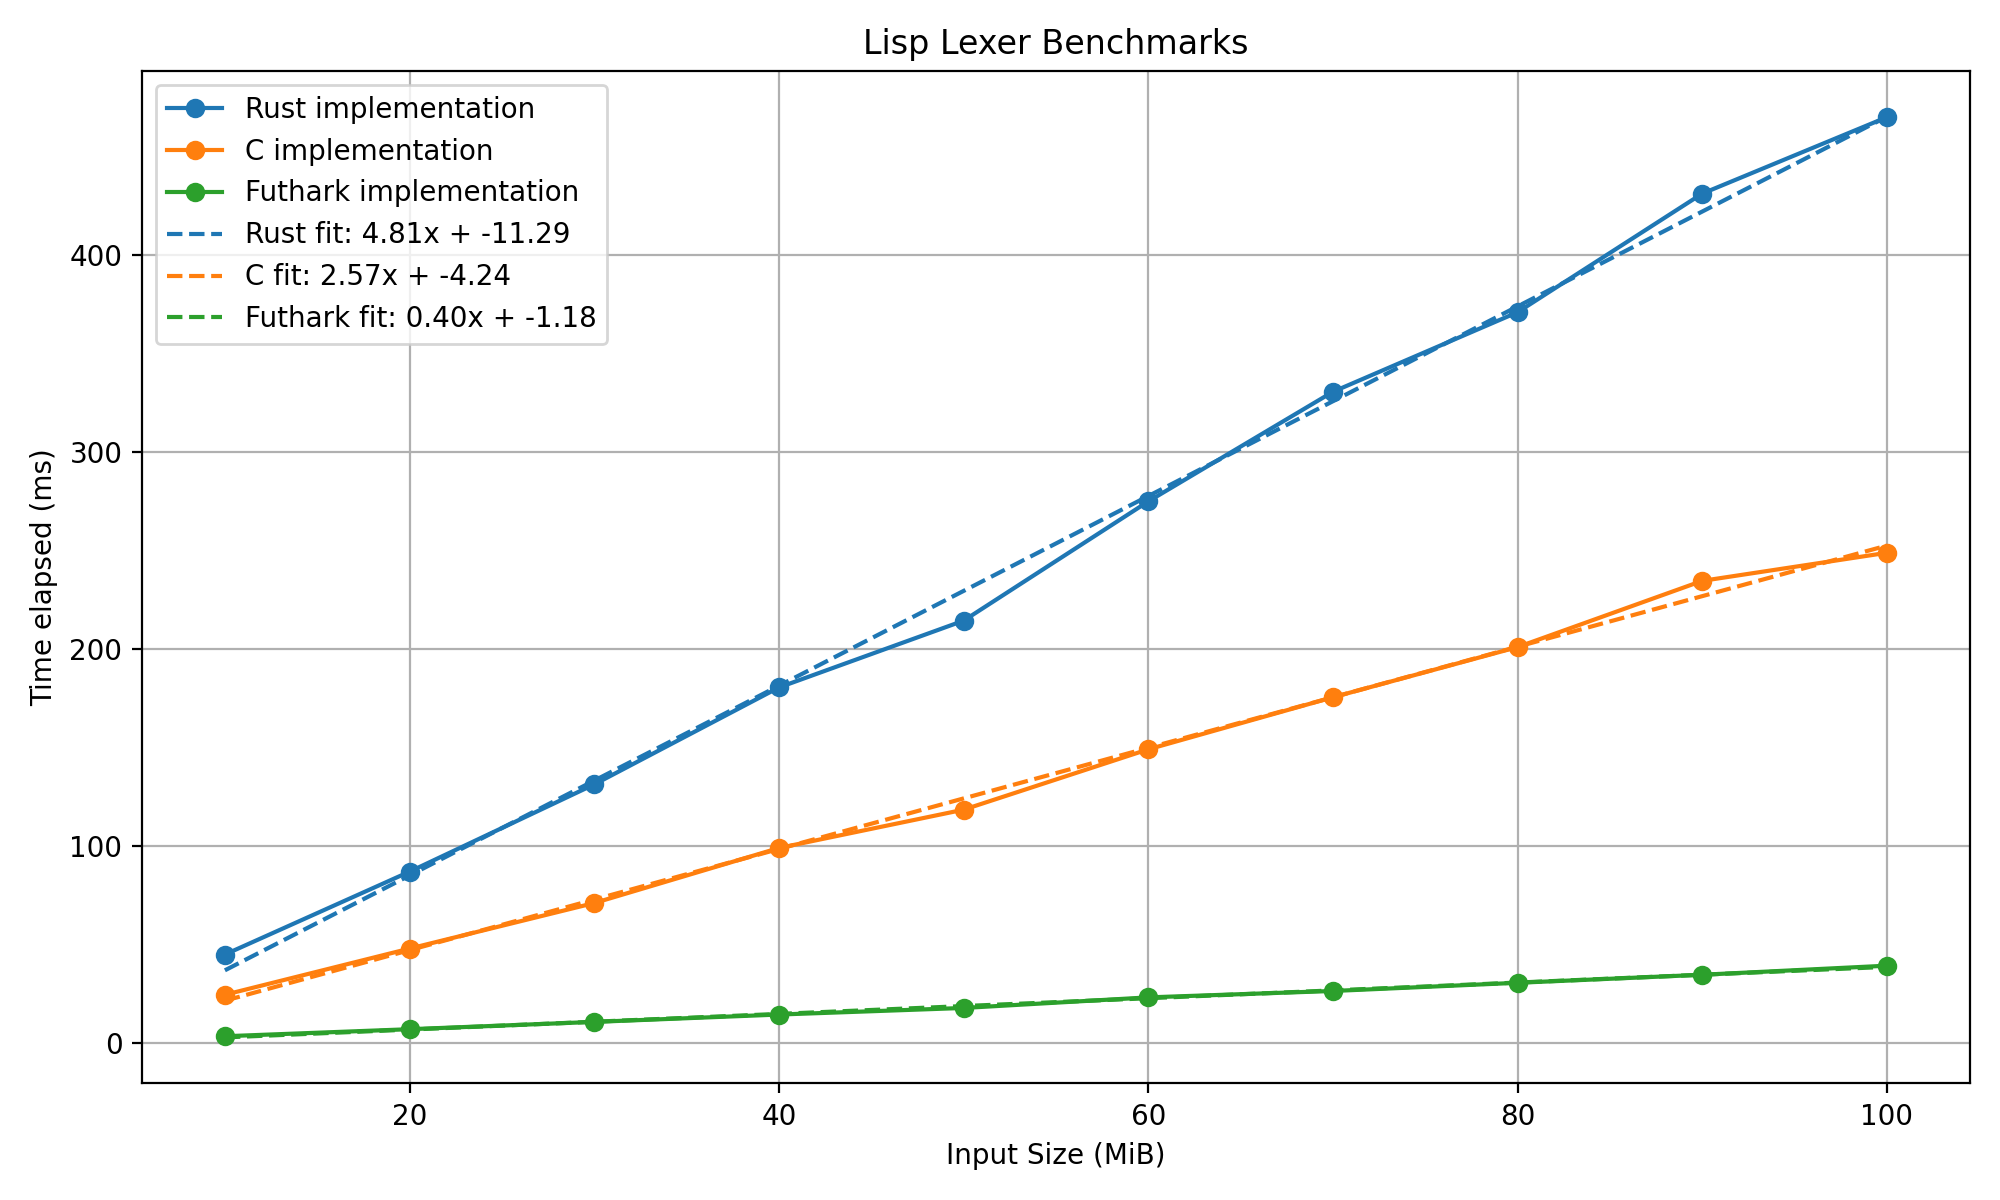
\includegraphics[width=\linewidth]{plot.png}
  \caption{Lisp Lexer Benchmarks}
\end{figure}
\noindent As we see from the plot the times grows roughly linearly with the input size for all the benchmarks. So we can use the linear equations found to solve for each lexers throughput in GiB/s.
\begin{table}[H]
  \centering
  \begin{tabular}{c|c|c|c}
     & Rust ($\mu s$) & C ($\mu s$) & Futhark ($\mu$s) \\ \hline
    Througput (GiB/s) & 0.2 & 0.4 & 2.5 \\
  \end{tabular}
  \caption{Lisp Lexers Throughput}
\end{table}

\section{Discussion}
As we see the the throughput of 
\section{Conclusion}
Conclusion.
\printbibliography
\end{document}